\section*{Exercice 189 -- TEC -- Clever}
\setcounter{exo}{0}
%Banque PT SI A 2013
On cherche à déterminer la masse équivalente $M_{eq}$ ramenée à la tige du vérin, de l'ensemble habitacle et mécanisme de transformation de mouvement actionnés par le vérin. Pour cela, on adopte les hypothèses suivantes :
\begin{itemize}
\item le référentiel associé au châssis \textbf{0} du véhicule Clever est supposé galiléen (ceci revient à supposer le châssis fixe par rapport au référentiel lié à la route durant la phase d'inclinaison) ;
\item la puissance dissipée engendrée par l'inclinaison de l'habitacle au niveau du contact roue/sol est négligée ;
\item les liaisons sont supposées parfaites.
\end{itemize}

Le modèle cinématique adopté est précisé par le schéma cinématique de la \autoref{fig_2_5}, ainsi que les données géométriques et les paramètres de mouvement. On note $m$ la masse de l'habitacle et $J_1 = \SI{175}{kg.m^{2}}$ son moment d'inertie par rapport à l'axe $\axe{O}{y_0}$. Les caractéristiques utiles des vérins sont données en annexe.

 % QUESTION 28
\subparagraph{}
\textit{Exprimer l'énergie cinétique galiléenne de l'ensemble des solides \{1,4,5\} en fonction des paramètres cinématiques  $\dot{\alpha}$,  $\dot{\theta}_1$ et  $\dot{\lambda}$.}
\ifprof
\begin{corrige}
\end{corrige}
\else
\fi




Pour simplifier la suite de l'étude, on se place autour de la position non-inclinée de l'habitacle. On définit alors le paramètre angulaire $\theta$ tel que $\theta = \theta_1 -\theta_{10}$. La figure du Cahier Réponses donne l'évolution du paramètre $\theta$ en fonction de $\lambda$. On cherche à linéariser cette fonction sous la forme $\theta = T\lambda$.

\begin{figure}[H]
\centering
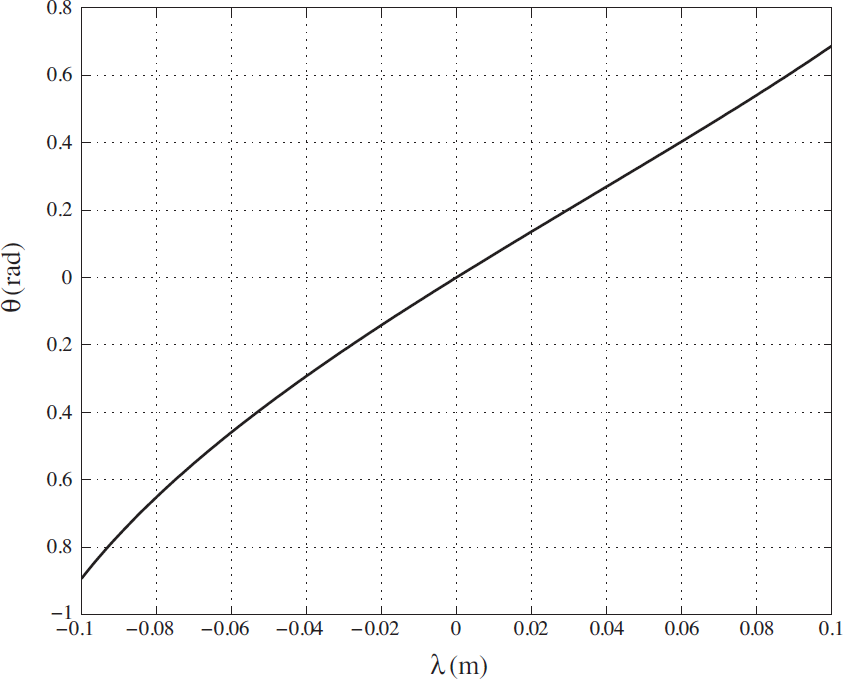
\includegraphics[width=\linewidth]{999_02}
%\label{fig_2_5}
%\caption{Schéma cinématique du modèle mécanique adopté}
\end{figure}

 % QUESTION 29
\subparagraph{}
\textit{Déterminer une valeur numérique approximative de $T$.}
\ifprof
\begin{corrige}
\end{corrige}
\else
\fi


Les valeurs numériques de $R$ et $T$ étant proches on prendra pour la suite du sujet : $R = T = \SI{7,5}{rad.m^{-1}}$.



\begin{figure}[H]
\centering
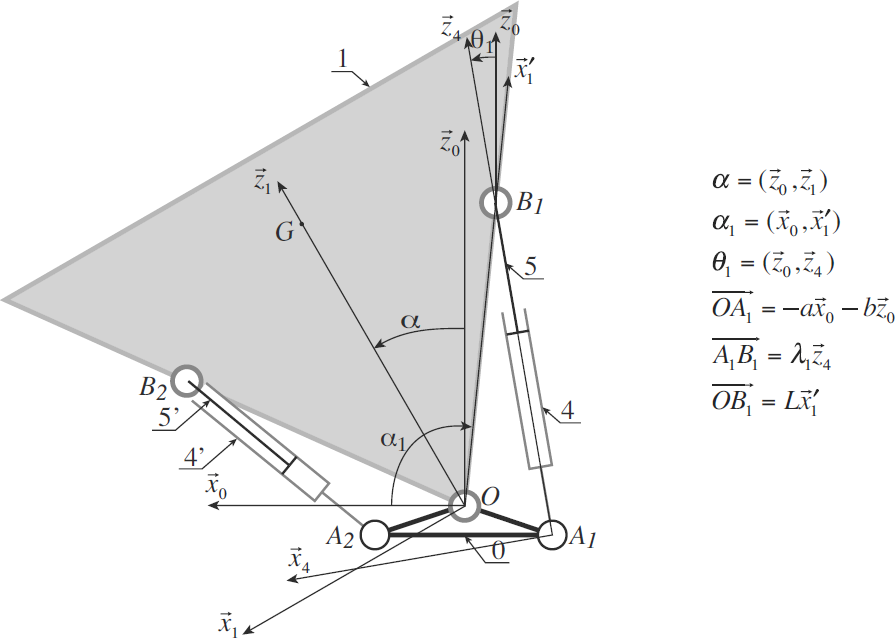
\includegraphics[width=\linewidth]{fig_2_5}
\label{fig_2_5}
\caption{Schéma cinématique du modèle mécanique adopté}
\end{figure}


\subparagraph{}
\textit{Exprimer la masse équivalente $M_{eq}$ ramenée à la tige du vérin en fonction des caractéristiques cinétiques des pièces et des paramètres géométriques en précisant clairement la méthode utilisée pour définir cette grandeur. À partir des données de l'Annexe A, montrer que les termes d'inertie liés aux 2 vérins sont faibles par rapport à celui associé à l'habitacle.}
\ifprof
\begin{corrige}
\end{corrige}
\else
\fi



\subparagraph{}
\textit{Appliquer le théorème de l'énergie cinétique à l'ensemble \{1,4,5\} en négligeant les termes dus aux puissances des poids de 4 et 5. Écrire le résultat sous la forme :
 $F_v + k_g \lambda = M_{eq} \ddot{\lambda}$ 
en donnant l'expression du paramètre $k_g$. Appliquer la transformation de Laplace à l'équation précédente et compléter le schéma-blocs du Cahier Réponses dans lequel la variable $V(p)$ correspond à  $\mathcal{L}\left(\dot{\lambda}(t)\right)$.}
\ifprof
\begin{corrige}
\end{corrige}
\else
\fi
